
Como ya adelantamos brevemente en la sección anterior, utilizamos Festvox y Festival para la generación de ``partituras'' necesarias en la síntesis de audios. A diferencia de las transcripciones fonéticas, estas transcripciones en realidad no se corresponden con ningún audio y son utilizadas por HTS para sintetizar habla. De alguna manera, actúan como una partitura para la generación acústica, indicándole a HTS qué fono debe sintetizar en cada momento. Es importante notar también, que los símbolos en las partituras y en las transcripciones utilizadas en el entrenamiento deben coincidir para que HTS pueda interpretarlas correctamente.  

Para la posterior combinación de modelos, se presenta aquí un desafío, ya que los repertorios fonéticos de estas partituras no tienen una correspondencia directa entre inglés y castellano. Por ejemplo con el repertorio fonético de Festvox en castellano, existen tres fonos distintos para la [i], decisión que proviene de la necesidad de poder diferenciar la [i] acentuada de la no acentuada  y de aquella presente en los diptongos [ia], [ie], [io], [iu]. La Tabla \ref{fig:foneRep} muestra los repertorios utilizados por Festvox para la generación de transcripciones fonéticas de castellano (con $31$ fonos) e inglés (con $40$ fonos).

\begin{table}
\centering
%\setlength{\tabcolsep}{6pt} % default value is 6pt
\begin{minipage}[t]{0.3\textwidth}
\begin{tabular}[t]{cc}
\toprule
Castellano \\
\midrule
a & m \\
a1 & n \\
b & ny \\
ch & o \\
d & o1 \\
e & p \\
e1 & r \\
f & rr \\
g & s \\
i & sp \\
i0 & t \\
i1 & th \\
k & u \\
l & u0 \\
ll & u1 \\
 & x \\
\bottomrule
\end{tabular}
\end{minipage}
\begin{minipage}[t]{0.3\textwidth}
\begin{tabular}[t]{cc}
\toprule
Inglés \\ 
\midrule
 aa & jh\\
 ae & k \\
 ah & l \\
 ao & m \\
 aw & n \\
 ax & ng\\
 ay & ow\\
 b  &oy\\
 ch & p \\
 d  &r \\
 s  &sh\\
 dh & t\\
 eh & th \\
 er & uh \\
 ey & uw \\
 f  &v\\
 g  &w\\
 hh & y\\
 ih & z\\
 iy & zh \\
\bottomrule
\end{tabular}
\end{minipage}
\caption{Repertorios fonéticos utilizados por Festvox para inglés y castellano} 
\label{fig:foneRep}
\end{table}

Como solución general, ideamos el siguiente método. Tomamos los fonos generados por Festival para el corpus en inglés y los traducimos a fonos del castellano antes del entrenamiento. Luego, entrenamos el modelo en inglés, utilizando los símbolos en castellano. De esta manera, esperamos construir un modelo en inglés capaz de comprender partituras que utilizan los símbolos en castellano.

El objetivo de esta sección será entonces generar una traducción de los fonos del inglés al castellano que nos permita junto con una partitura en castellano y un corpus en inglés, sintetizar habla en castellano.

Para ello, confeccionamos una tabla donde cada fono del repertorio del castellano estuviera mapeado a uno del repertorio del inglés. Por ejemplo el fono [ae] (\textit{alice}) del inglés lo traducimos al fono [a] (\textit{amigo}) del castellano. De la misma manera, el fono [ao] del inglés (\textit{for}) pasa a ser el fono [o] (\textit{gato}) del castellano. En la Tabla \ref{mapeoFonetico} se presenta una lista exhaustiva de los reemplazos fonéticos utilizados.

\begin{table}
\centering
%\setlength{\tabcolsep}{6pt} % default value is 6pt
\caption{Mapeo Fonético}
\label{mapeoFonetico}
\begin{minipage}[t]{0.3\textwidth}
\begin{tabular}[t]{c|c}
\toprule
Inglés & Castellano \\
\midrule
ae &	a \\
aa &	a1 \\
b &	b \\
ch &	ch \\
d &	d \\
dh &	d \\
eh &	e \\
el &	e1 \\
f &	f \\
hh & g \footnotemark\\
iy &	i \\
%falta  i0
ih &	i1 \\
k &	k \\
l &	l \\
jh &	ll \\
m &	m \\
n &	n \\
nx &	n \\
n + i &  ny \\
ao &	o \\
ou &	o1 \\
\bottomrule
\end{tabular}
\end{minipage}
\begin{minipage}[t]{0.3\textwidth}
\begin{tabular}[t]{c|c}
\toprule
Inglés & Castellano \\ 
\midrule
p &	p \\
r &	r/rr \\
%falta x
s &	s \\
t &	t \\
uw &	u \\
w &	u0 \\
uh &	u1 \\
g &	-\\
dx &- \\
em &- \\
en &- \\
er &- \\
ei &- \\
hv &- \\
ng &- \\
th &- \\
v & -\\
y & -\\
sh &- \\
zh &- \\
z & - \\ 

\bottomrule
\end{tabular}
\end{minipage}
\end{table}

\footnotetext{El mapeo de [hh] a [g] en castellano resultó ser incorrecto. El fono [g] existe tanto en castellano (\textit{gato}) como en inglés (\textit{glad}). Notamos este error recién al hacer la evaluación perceptual, como se describe en la Sección \ref{datosNormalizados}.}

Por otro lado, para varios fonos tuvimos que hacer reglas especiales ya que no contábamos con ningún fono del inglés lo suficientemente similar. Así,  para el fono ny (ñ o \textltailn, en ipa) colapsamos las apariciones del fono [n] seguido de [i]. Si bien esta solución puede parecer algo forzada, ya que estamos generando de manera casera un fono a partir de otros dos, consideramos que esto se aproxima en cierta medida a la manera real en la que un hablante no nativo aprende un idioma con una carga fonética diferente a la suya. Citando un extracto del trabajo \textit{Transcription of Spanish and Spanish-Influenced English, Brian Goldstein, Temple University} \cite{spanishInfluencedEnglish}:

\begin{figure}[H]
\centering
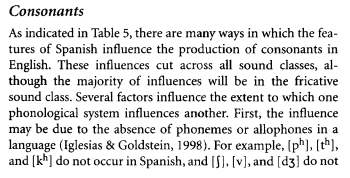
\includegraphics[scale=0.6]{imagenes_investigacion/consonantes1.png}
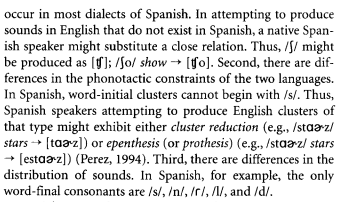
\includegraphics[scale=0.6]{imagenes_investigacion/consonantes2.png}
\end{figure}

Es decir, visto desde nuestra perspectiva, una persona que aprende una nueva lengua, realiza una aproximación entre los fonos conocidos y los fonos `objetivo' de la nueva lengua. Esta perspectiva nos alienta a realizar mapeos que no resultan del todo exactos, mapeando por ejemplo el fono [w] (\textit{twentieth}) del inglés al fono [u0] (\textit{cuatrimestre}) del castellano o el fono [uw] (\textit{two}) por el fono [u] (\textit{cumplió}).

Un mapeo que podría resultar controversial es el del fono [jh] (\textit{danger}) del inglés por el [ll] (\textit{billete}) del castellano, porque existen otras posibilidades: podría mapearse a [sh] (ash), por ejemplo. Sin embargo, consideramos que el mapeo elegido es el que más se acerca a la pronunciación de las locutoras de las grabaciones.

De manera similar, el inglés carece del fono vibrante múltiple alveolar sordo [\textipa{r}] (\textit{perro}) y dado que el fono [\textipa{R}](\textit{pero})  ya está siendo utilizado, no podemos mapearlo a este. Es importante reiterar aquí que no podemos dejar sin cubrir ningún fono del castellano ya que entonces el modelo generado no sería completamente compatible con la partitura en castellano. 

Para hacer hincapié en el problema, supongamos que el fono [\textipa{r}] queda sin cubrir por ningún fono del inglés. Entrenamos el modelo con el corpus de inglés, reemplazando los símbolos del inglés por los del castellano. Ahora le damos para sintetizar una partitura con símbolos en castellano donde se encuentra presente el fono [\textipa{r}]. El modelo no tendrá manera de inferir el sonido correcto para este símbolo, resultando en una síntesis errónea o de baja calidad. 

Una solución que encontramos para este problema es mapear cada ocurrencia de [\textipa{R}] en inglés con equiprobabilidad a [\textipa{R}] o a [\textipa{r}] en castellano. De esta manera ambos símbolos del castellano quedan cubiertos por el símbolo más similar del inglés.

Aquellos fonos del inglés que consideramos suficientemente disímiles del castellano, como es el caso de la [sh] y [z] los mapeamos a caracteres que no interfirieran para el entrenamiento ya que no los utilizaremos para la síntesis de oraciones en castellano.

Con este mapeo, podemos utilizar el corpus en inglés para sintetizar oraciones con partituras en castellano. Sin embargo, como es de esperar, los audios sintetizados resultan incomprensibles, por cuestiones como que las combinaciones de fonos del inglés y el castellano son muy distintas, así como las reglas prosódicas y las acentuaciones de las palabras, entre otras marcadas diferencias.

% mapeo utilizado mostrar.
% el etiquetado de cmu\_arctic es en inglés y mapeando al castellano.